\section{Reference Approach}
\label{sec:reference}
In this section, we introduce the $\Reference$ approach~\cite{MATLAB:reference} used later (see \cref{sec:results}) for comparison.
According to \cref{eq:refEquation}, the memory footprint $\MemF$ is linear in $k$, the number of breakpoints.
An obvious remaining problem here is how to determine an equidistant spacing $\Spacing{ }$ being as large as possible such that still a user-given maximal approximation error bound $\AbsError$ is never exceeded for any evaluation of $\Fx$ inside the given interval $[\LowerBound, \UpperBound)$.
Let $p_i(x)$ denote the linear polynomial used to approximate the function $\Fx$ between the adjacent breakpoints $[\Breakpoint{i},\Breakpoint{i+1})$.
A two-point line expression can be derived from \cref{eq:linEq} as follows: 
\begin{equation}
p_i(x)=p_i(x_i)+\frac{x-x_i}{x_{i+1}-x_i}(p_i(x_{i+1})-p_i(x_i))
\label{eq:one}
\end{equation}
If the second derivative $f''(x)$ of $\Fx$ does exist at each point in $[x_i,x_{i+1})$, then the difference between the exact function value $\Fx$ and the value of the approximating polynomial $p_i(x)$ in $x_i \leq x < x_{i+1}$ is given as:
\begin{equation}
\Fx-p_i(x)=\frac{(x-x_i)(x-x_{i+1})}{2} f''(\varepsilon_x)
\label{eq:two}
\end{equation}
In \cref{eq:two}, $\varepsilon_x$ is some value between  $x_i$ and $x_{i+1}$.
In consequence, an error bound can be formulated based on \cref{eq:one,eq:two} as:
\begin{equation}
|\Fx-p_i(x)| \leq \frac{(x-x_i)(x_{i+1}-x)}{2} \max_{x_i\leq x < x_{i+1}} |f''(x)|
\label{eq:three}
\end{equation} 
With the spacing $\Spacing{i}=\Breakpoint{i+1}-\Breakpoint{i}$ between $\Breakpoint{i}$ and $\Breakpoint{i+1}$, the maximum value of $(x-x_i)(x_{i+1}-x)$ in \cref{eq:three} can be constrained as:
\begin{equation}\label{eq:four} 
\max_{x_i \leq x< x_{i+1}} (x-x_i)(x-x_{i+1}) = \frac{\Spacing{i}^2}{4}
\end{equation}
By combining \cref{eq:three,eq:four}, we obtain a maximum approximation error bound $E_i$ given a spacing $\Spacing{i}$:
\begin{equation}\label{eq:five}
E_i = \frac{\delta_i^2}{8} \max_{x_i\leq x < x_{i+1}} |f''(x)|
\end{equation}
The dependence of the approximation error on the second derivative of a function is intuitive from the perspective of linearity.
If $f$ is truly linear in the interval $[x_i,x_{i+1})$, then the second derivative vanishes implying an exact representation.
The value of $\underset{x_i\leq x <x_{i+1}}{\max} |f''(x)|$ can be expressed in closed form for elementary functions as well as some of the non-elementary functions due to their well-defined second derivatives.
Finally, for a given user-defined maximal approximation error bound $\AbsError$ to hold between any pair of breakpoints and assuming equi-distant spacings $\delta = \delta_i, 0 \leq i \leq k-1$, we can infer the biggest permissible spacing $\delta$ from the segment $i$ with the smallest value of $\Spacing{i}$ in \cref{eq:five}:
\begin{equation}\label{eq:spacing_err}
\delta(f,\AbsError,[\Breakpoint{0},\Breakpoint{k}))=\underset{0 \leq i \leq k-1}{\min} \bigg( 8\cdot \frac{\AbsError}{\underset{x_i\leq x < x_{i+1}}{\max} |f''(x)|} \bigg )^{\frac{1}{2}}
\end{equation}
\begin{figure}[t!]
	\centering
	\begin{subfigure}[b]{\textwidth}
		\centering
		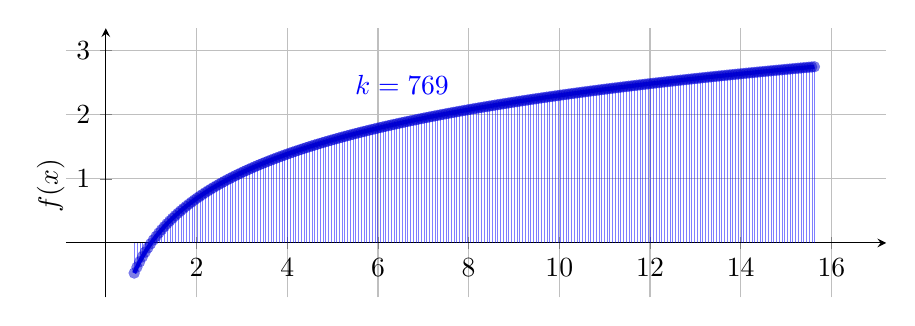
\begin{tikzpicture}[scale=1]
		\pgfplotsset{%compat=1.14,         
			width=12cm,     
			height=5cm, 
		}
		\begin{axis}[grid=both,
		ymin=-0.5,
		xmax=15.7,ymax=3,
		axis lines=middle,
		enlargelimits,
		ylabel=$f(x)$,
		ylabel style={rotate=90,xshift=-2cm,yshift=1cm},
		]
		\addplot+[ycomb,line width=0.05pt,domain=0.625:15.625,samples=250,opacity=0.5] {ln(x)};
		\addplot[black,mark=none,line width=1.5pt,domain=0.625:15.625,samples=400,color=blue]  {ln(x)} node[above left,yshift=-0.5cm,xshift=-4.5cm] {$k=769$};
		\end{axis}
		\end{tikzpicture}
		\caption{\label{fig:entries}Table-based approximation of $f(x)=log(x)$. Here, $\Spacing{}=0.019$, resulting in a memory footprint of $\MemF=k+1=770$ entries.}
	\end{subfigure}
	\begin{subfigure}[b]{\textwidth}
		\centering
		\begin{tikzpicture}[scale=1]
		\pgfplotsset{%compat=1.14,         
			width=12cm,     
			height=5cm, 
		}
		\begin{axis}[grid=both,
		axis lines=middle,
		enlargelimits,
		ylabel = $E$,
		ylabel style={rotate=90,xshift=-1.7cm,yshift=1cm,},
		%yshift=-1cm
		]
		\addplot[samples=16000,black,mark=none,line width=0.05pt,color=ao] table[x=x,y=y] {tikz/errormargins.dat};
		\draw[very thick, densely dashed,draw=red] (axis cs: 0,1.25E-4) --node[below,color=red]{\small $\AbsError$} (axis cs:15.625,1.25E-4);
		\end{axis}
		%\node[rotate=90] at (-0.5,1.5) {$E$};
		\end{tikzpicture} 
		\caption{\label{fig:ErrorMargin}Approximation Error obtained using \cref{eq:spacing_err} given $\AbsError=1.25E-04$.}
	\end{subfigure}
	\caption{\label{fig:tabApp} Function approximation of $\Fx=log(x)$ in the interval $[0.625,15.625)$. }
\end{figure}
E.g., \cref{fig:tabApp} illustrates the approximation of $\Fx=log(x)$ in the interval $[0.625,15.625)$ and $\AbsError=1.25E-04$.
This results in an spacing $\Spacing{}(log(x),\AbsError,[0.625,16.625))=0.019$.
From a spacing $\Spacing{}$ and the interval $[\LowerBound,\UpperBound)$, it is possible to generate the entries to be stored in a lookup table (see \cref{fig:entries}).
Given a spacing $\Spacing{}$  and an interval $[\LowerBound,\UpperBound)$, the memory footprint of this approach called $\Reference$ approach in the following can be calculated as:
\begin{equation}
\MemF^R(\Spacing{},[\LowerBound,\UpperBound)) = \bigg\lceil \dfrac{\UpperBound-\LowerBound}{\Spacing{}} \bigg\rceil + 1
\label{eq:six}
\end{equation}
Thus, the memory footprint of $\Fx=log(x)$, given the interval $[0.625,15.625)$, and $\Spacing{}=0.019$ is $\MemF^R(0.019,[0.626,15.625)) = 770$ entries.\\
The $\Reference$ approach performs the function approximation given a maximum approximation error $\AbsError$ by delivering a set of evenly spaced breakpoints.
However, this approach does not take into account the gradient in different regions of the interval.
This may result in an inefficient footprint, e.g., in \cref{fig:tabApp}, the interval closest to the left-most point $x_0=0.625$ determines the maximal spacing for the given approximation error $\AbsError$.
However, it can be seen that for larger values of $x$ (see \cref{fig:ErrorMargin}), a coarser spacing could be used when splitting the domain into sub-intervals and using different spacings $\delta_i$ within these.
Our main idea for the three proposed approaches introduced in the following is therefore to use different spacings $\delta_i$ by splitting the given interval into sub-intervals.
